\documentclass[tikz,border=2pt]{standalone}
\usepackage{amsmath,amssymb}
\usepackage{tikz}
\usepackage{pgfplots}
\pgfplotsset{compat=1.18}

\begin{document}
% Integer demand (dress example): beta = 0.75, F(9) = 0.70 < 0.75 <= F(10) = 0.85, so the
% smallest optimal quantity is 10; the other steps of the CDF are drawn schematically.
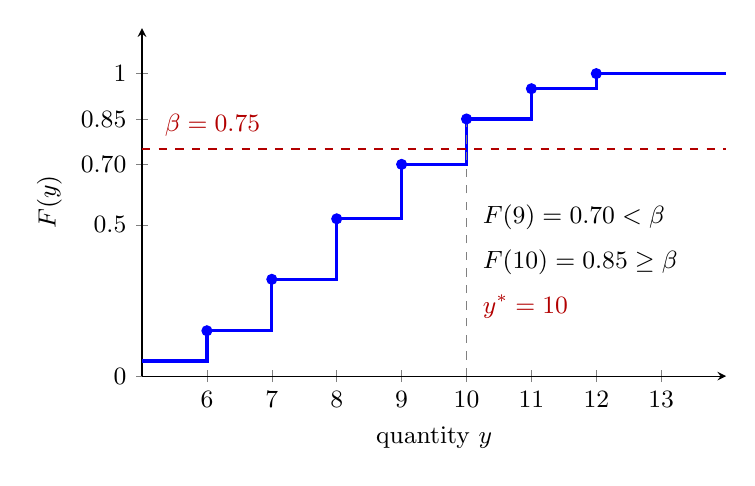
\begin{tikzpicture}
	\begin{axis}[width=9cm, height=6cm, xlabel={quantity $y$}, ylabel={$F(y)$}, xmin=5, xmax=14, ymin=0, ymax=1.15, axis lines=left, tick label style={font=\small}, label style={font=\small}, xtick={6,7,8,9,10,11,12,13}, ytick={0,0.5,0.70,0.85,1}, yticklabels={0,0.5,0.70,0.85,1}]
		\addplot[blue, very thick, const plot] coordinates {(5,0.05) (6,0.15) (7,0.32) (8,0.52) (9,0.70) (10,0.85) (11,0.95) (12,1) (14,1)};
		\addplot[only marks, mark=*, mark size=1.8pt, blue] coordinates {(6,0.15) (7,0.32) (8,0.52) (9,0.70) (10,0.85) (11,0.95) (12,1)};
		\draw[red!70!black, dashed, thick] (axis cs:5,0.75) -- (axis cs:14,0.75);
		\node[anchor=south west, font=\small, red!70!black] at (axis cs:5.2,0.76) {$\beta=0.75$};
		\draw[gray, dashed] (axis cs:10,0) -- (axis cs:10,0.85);
		\node[anchor=north west, font=\small] at (axis cs:10.1,0.6) {$F(9)=0.70<\beta$};
		\node[anchor=north west, font=\small] at (axis cs:10.1,0.45) {$F(10)=0.85\ge\beta$};
		\node[anchor=north west, font=\small, red!70!black] at (axis cs:10.1,0.3) {$y^*=10$};
	\end{axis}
	\end{tikzpicture}
\end{document}
